%%%%%%%%%%%%%%%%%%%%%%%%%%%%%%%%%%%%%%%%%%%%%%%%%%%%%%%%%%%%%
% Wireframe Design Section
%%%%%%%%%%%%%%%%%%%%%%%%%%%%%%%%%%%%%%%%%%%%%%%%%%%%%%%%%%%%%

\section{Wireframe}
การสร้าง wireframe เป็นขั้นตอนสำคัญในกระบวนการออกแบบเว็บหรือแอบพลิเคชัน เนื่องจากช่วยให้ทีมออกแบบและผู้เกี่ยวข้องเข้าใจโครงสร้างพื้นฐานของหน้าจอและการจัดวางองค์ประกอบหลัก ๆ โดยไม่จำเป็นต้องใส่รายละเอียดกราฟิกหรือสี นอกจากนี้ยังช่วยทำให้เห็นถึงภาพรวมประสบการณ์ผู้ใช้
ทำให้สามารถทดสอบและปรับปรุงก่อนที่จะเริ่มการพัฒนา และทำให้กระบวนการออกแบบเป็นไปอย่างมีประสิทธิภาพและรวดเร็วขึ้น โดยเราเลือกที่จะสร้าง wireframe ในส่วนที่เป็นฟีเจอร์สำคัญเพื่อที่จะสามารถนำไปทดสอบกับผู้ใช้ในกระบวนการคิดเชิงออกแบบ (Design Thinking)
\subsection {Resume Checker}
\label{subsec:ResumeChecker}
Resume Checker เป็นฟีเจอร์ที่ให้ผู้ใช้กรอกข้อมูลของเพื่อนำไปวิเคราะห์อาชีพที่เหมาะสม โดยผู้ใช้สามารถการข้อมูลเกี่ยวกับประสบการณ์ทำงาน, การศึกษา, ทักษะ, และคุณสมบัติอื่น ๆ ที่สำคัญ
\begin{itemize}
    \item หน้าหลัก
          \begin{figure}[H]\centering
              \setlength{\fboxrule}{0.2mm} % can define this in the preamble
              \setlength{\fboxsep}{0.5cm}
              \fbox{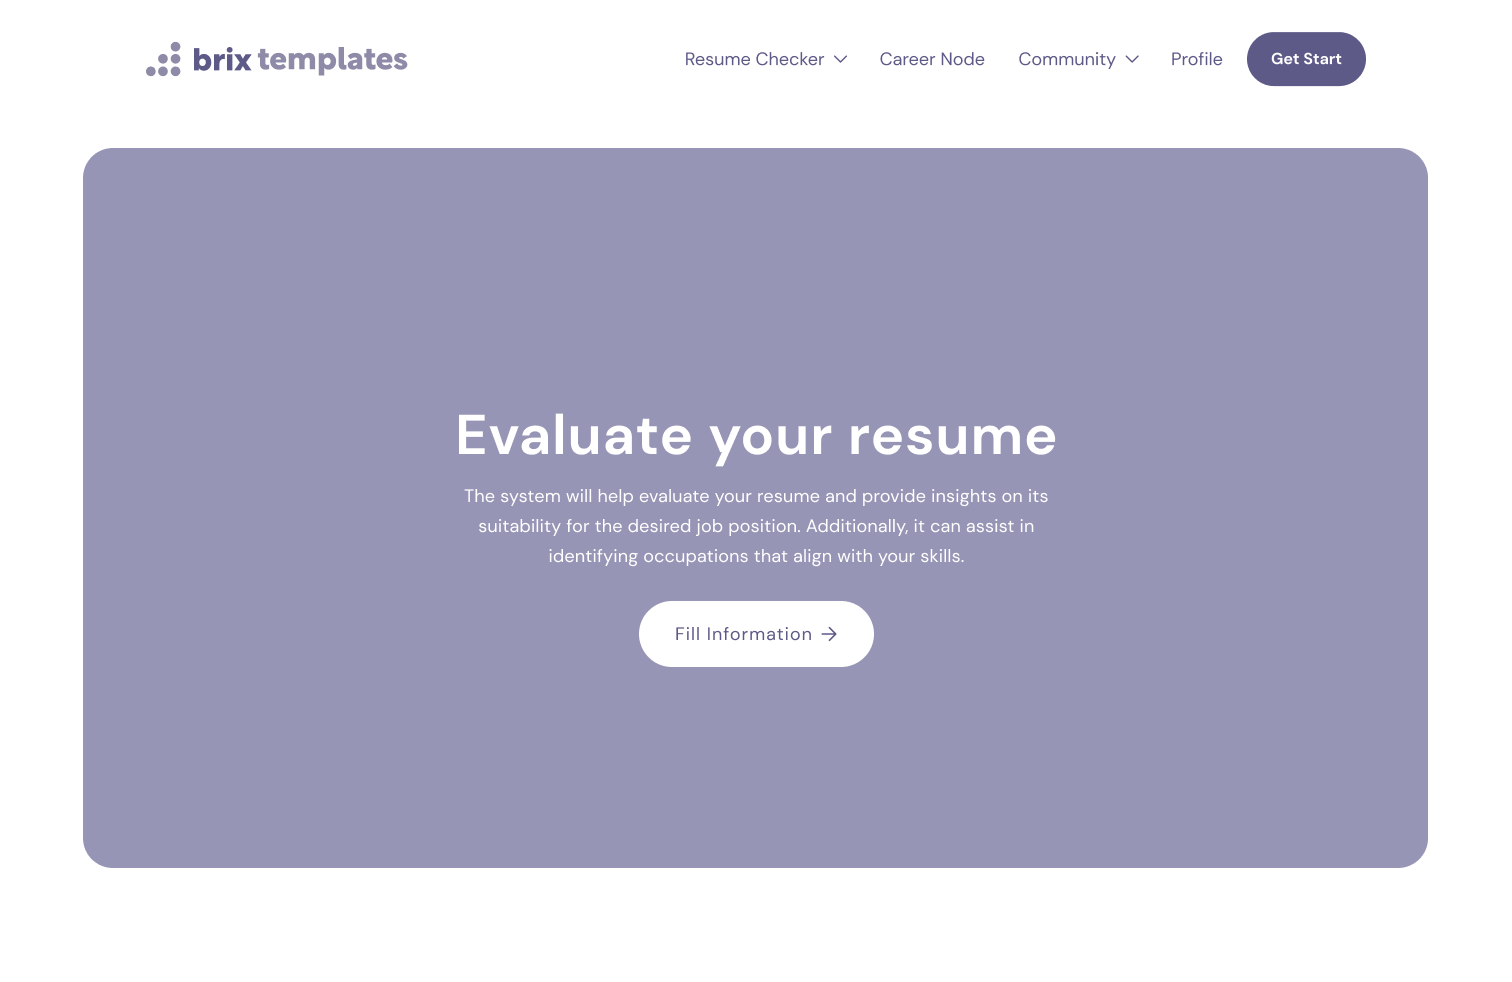
\includegraphics[width=8cm]{./figure/figure_wireframe_table1_mainpage1.png}}
              \caption{\centering หน้าหลักสำหรับกดเริ่มวิเคราะห์ Resume}\label{fig:wireframe1_1}
          \end{figure}
          \begin{figure}[H]\centering
              \setlength{\fboxrule}{0.2mm} % can define this in the preamble
              \setlength{\fboxsep}{0.5cm}
              \fbox{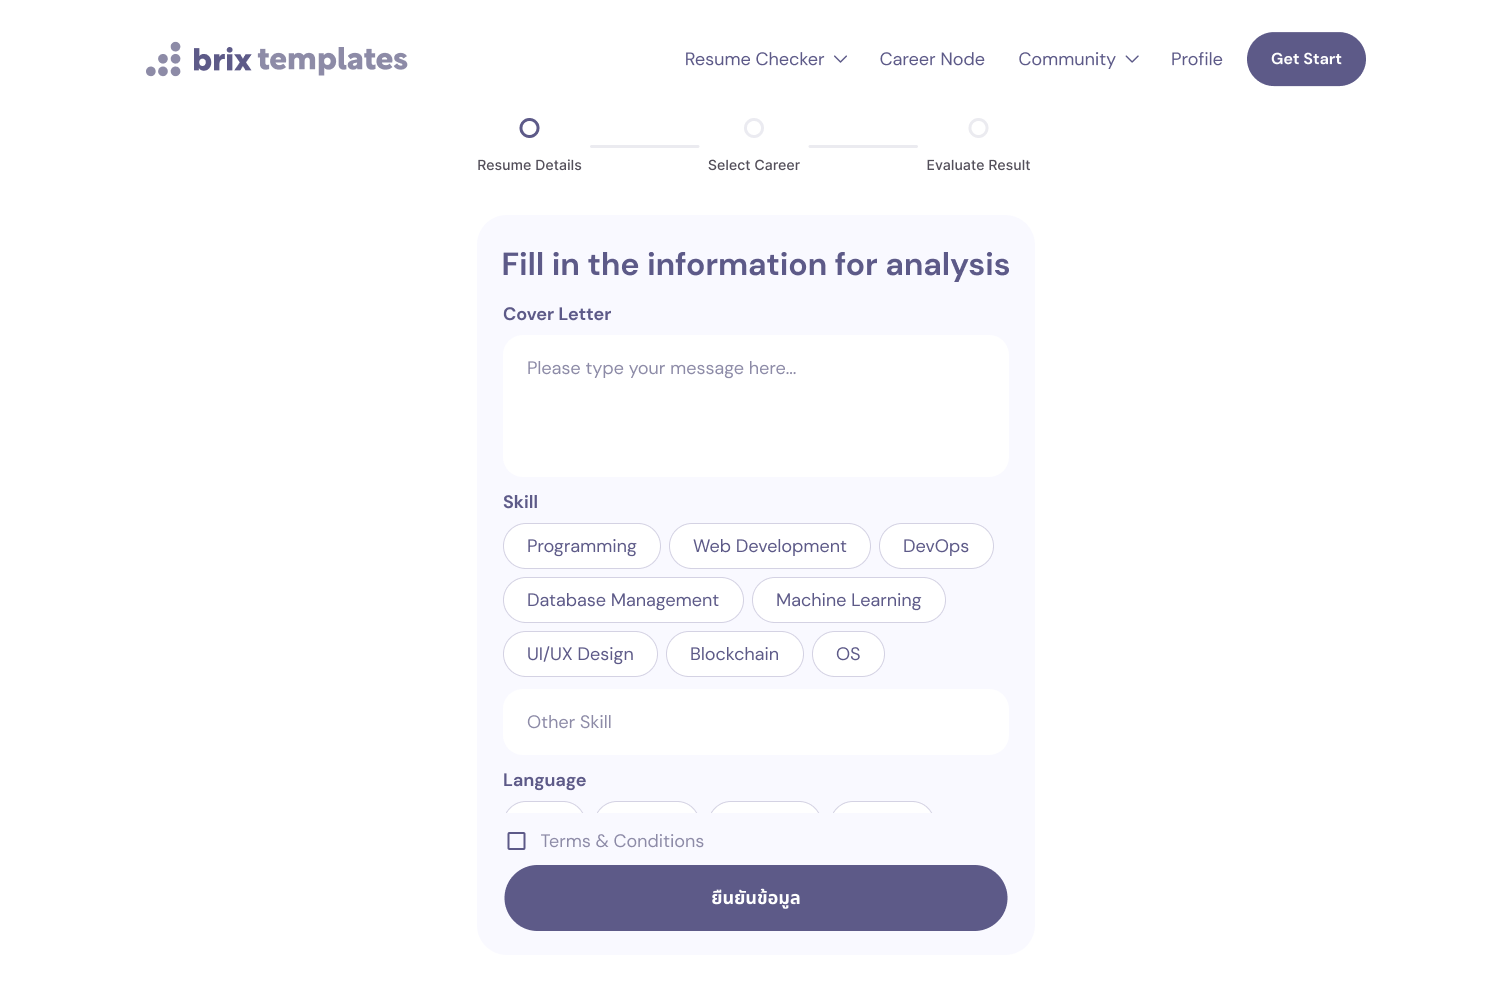
\includegraphics[width=8cm]{./figure/figure_wireframe_table1_mainpage2.png}}
              \caption{\centering หน้ากรอกข้อมูลของเพื่อนำไปวิเคราะห์}\label{fig:wireframe1_2}
          \end{figure}
    \item ส่วนประกอบแบบโต้ตอบ
          \begin{figure}[H]\centering
              \setlength{\fboxrule}{0.2mm} % can define this in the preamble
              \setlength{\fboxsep}{0.5cm}
              \fbox{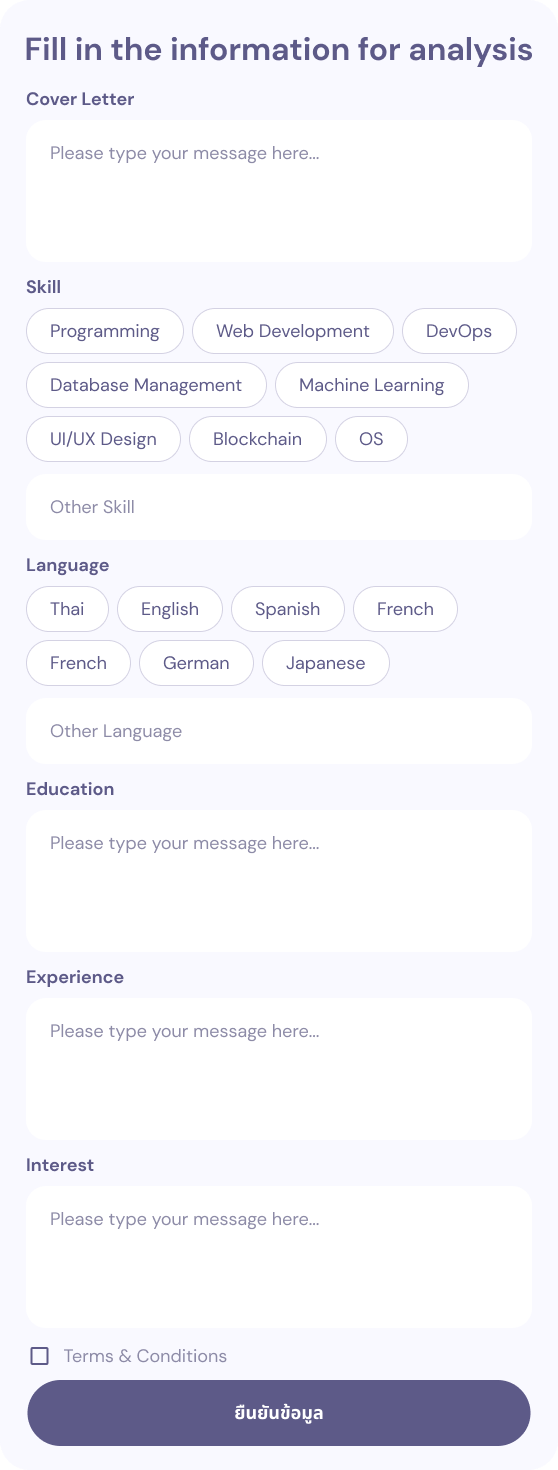
\includegraphics[width=8cm]{./figure/figure_wireframe_table1_component1.png}}
              \caption{\centering ช่องสำหรับกรอกข้อมูลของเพื่อนำไปวิเคราะห์}\label{fig:wireframe1_3}
          \end{figure}
\end{itemize}

\subsection {Match Career}
Match Career เป็นฟีเจอร์สำหรับแสดงอาชีพที่เหมาะสมกับข้อมูลที่ผู้ใช้กรอกมาทำให้ผู้ใช้สามารถรู้ถึงอาชีพที่เหมาะสมกับตนเองและข้อมูลคร่าว ๆ ของอาชีพนั้น โดยผู้ใช้สามารถกลับไปแก้ไขข้อมูลที่กรอกได้เพื่อนำมาวิเคราะห์อาชีพใหม่ รวมถึงสามารถกดวิเคราะห์ข้อมูลเชิงลึกต่อไปได้แต่ผู้ใช้ต้องสมัครและล็อคอินเพื่อเก็บข้อมูลก่อน
\begin{itemize}
    \item หน้าหลัก
          \begin{figure}[H]\centering
              \setlength{\fboxrule}{0.2mm} % can define this in the preamble
              \setlength{\fboxsep}{0.5cm}
              \fbox{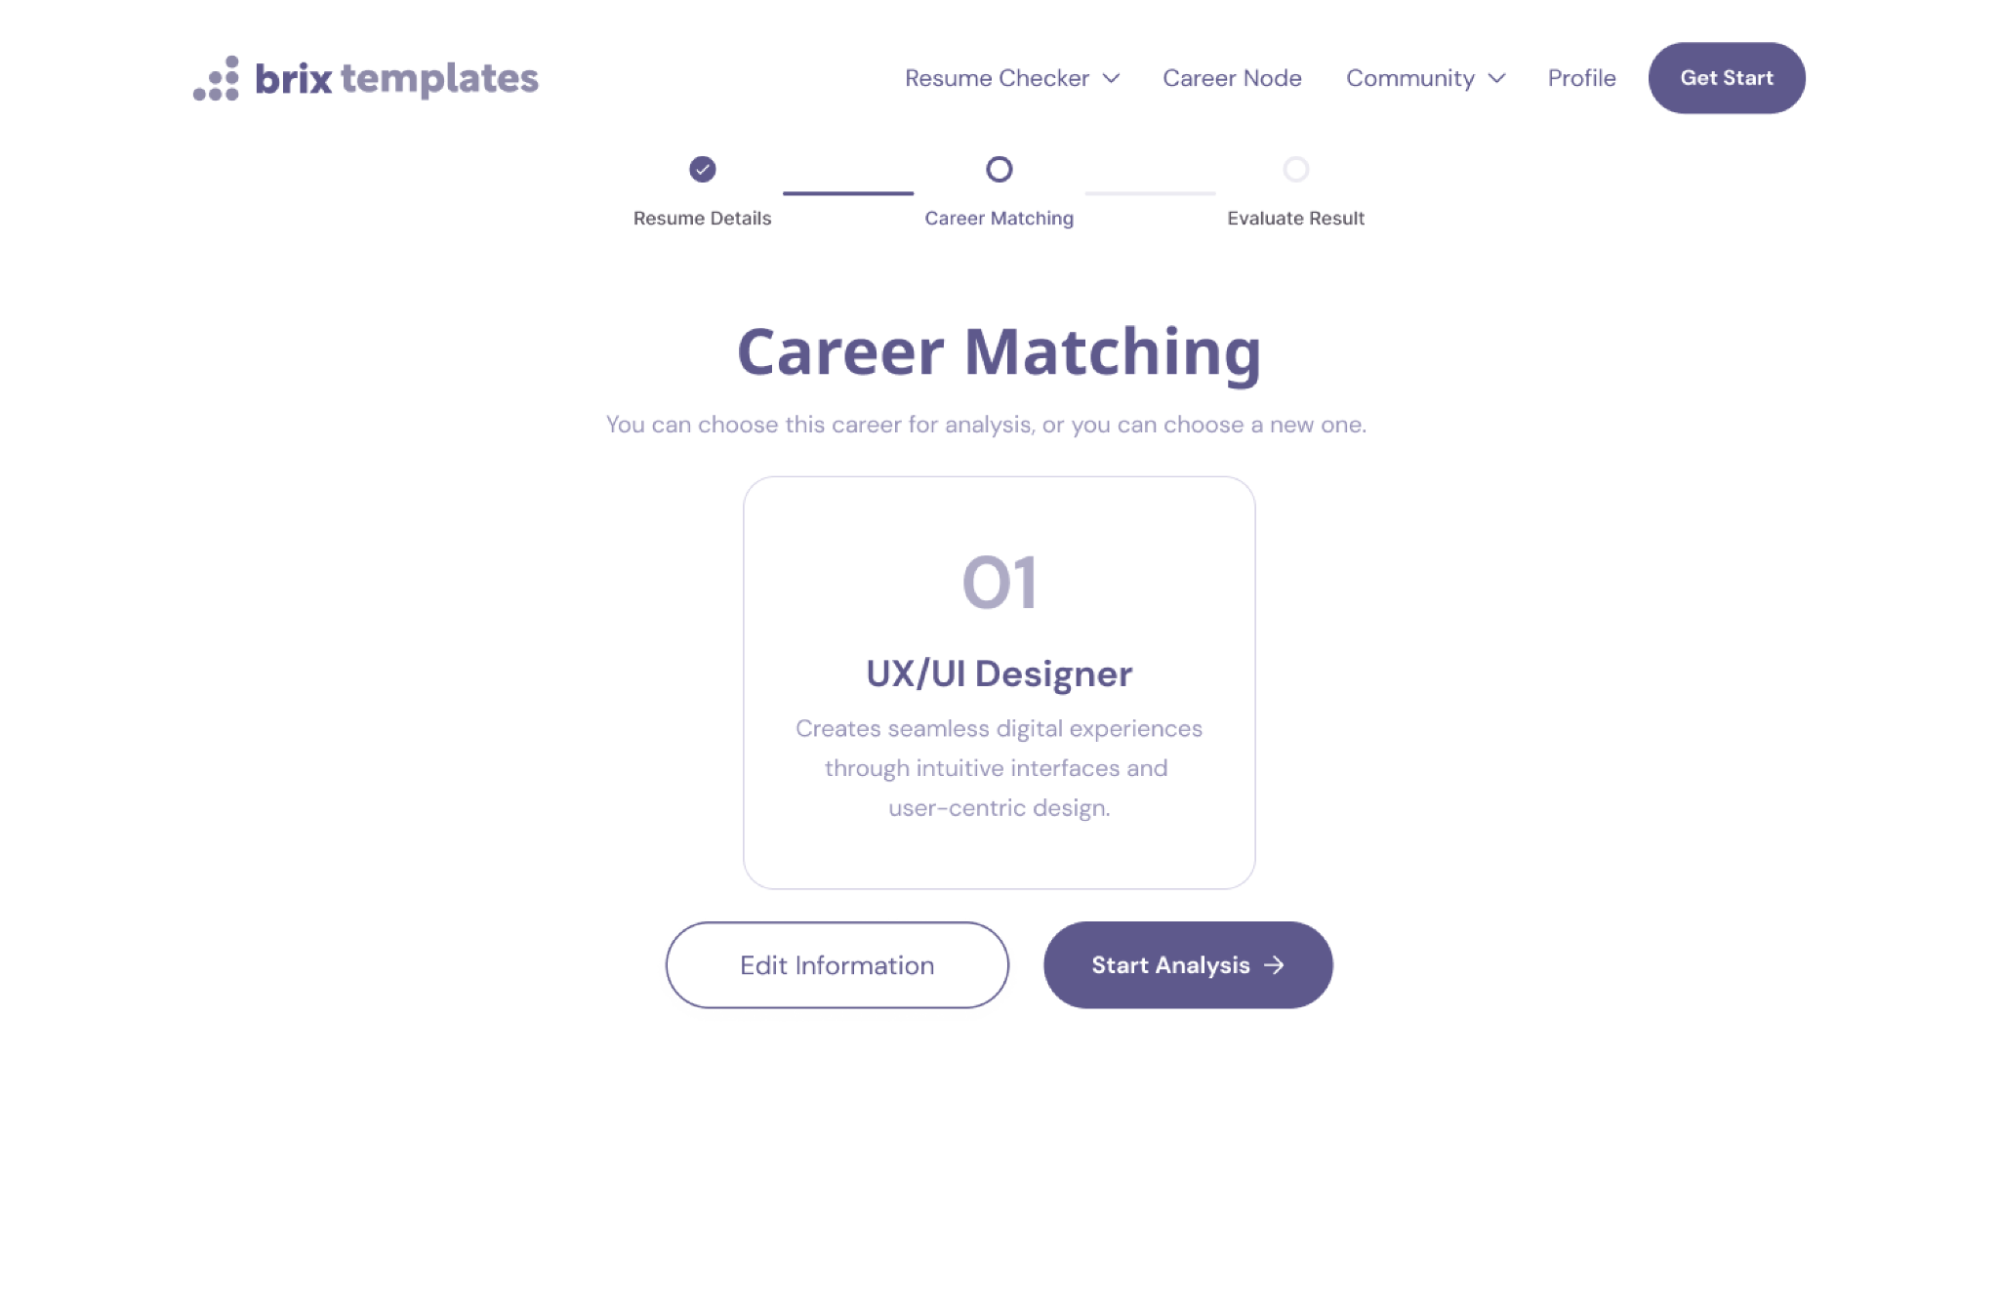
\includegraphics[width=8cm]{./figure/figure_wireframe_table2_mainpage1.png}}
              \caption{\centering หน้าแสดงอาชีพที่วิเคราะห์ได้}\label{fig:wireframe2_1}
          \end{figure}
\end{itemize}

\subsection {Evaluate Result}
Evaluate Result เป็นฟีเจอร์สำหรับแสดงข้อมูลเชิงลึกของอาชีพที่วิเคราะห์ได้ในตอนแรก โดยจะแสดงข้อมูลที่มีโยชน์เพื่อให้ผู้ใช้สามารถนำไปพัฒนาทักษะของตนเองและเรซูเมต่อไปได้
\begin{itemize}
    \item หน้าหลัก
          \begin{figure}[H]\centering
              \setlength{\fboxrule}{0.2mm} % can define this in the preamble
              \setlength{\fboxsep}{0.5cm}
              \fbox{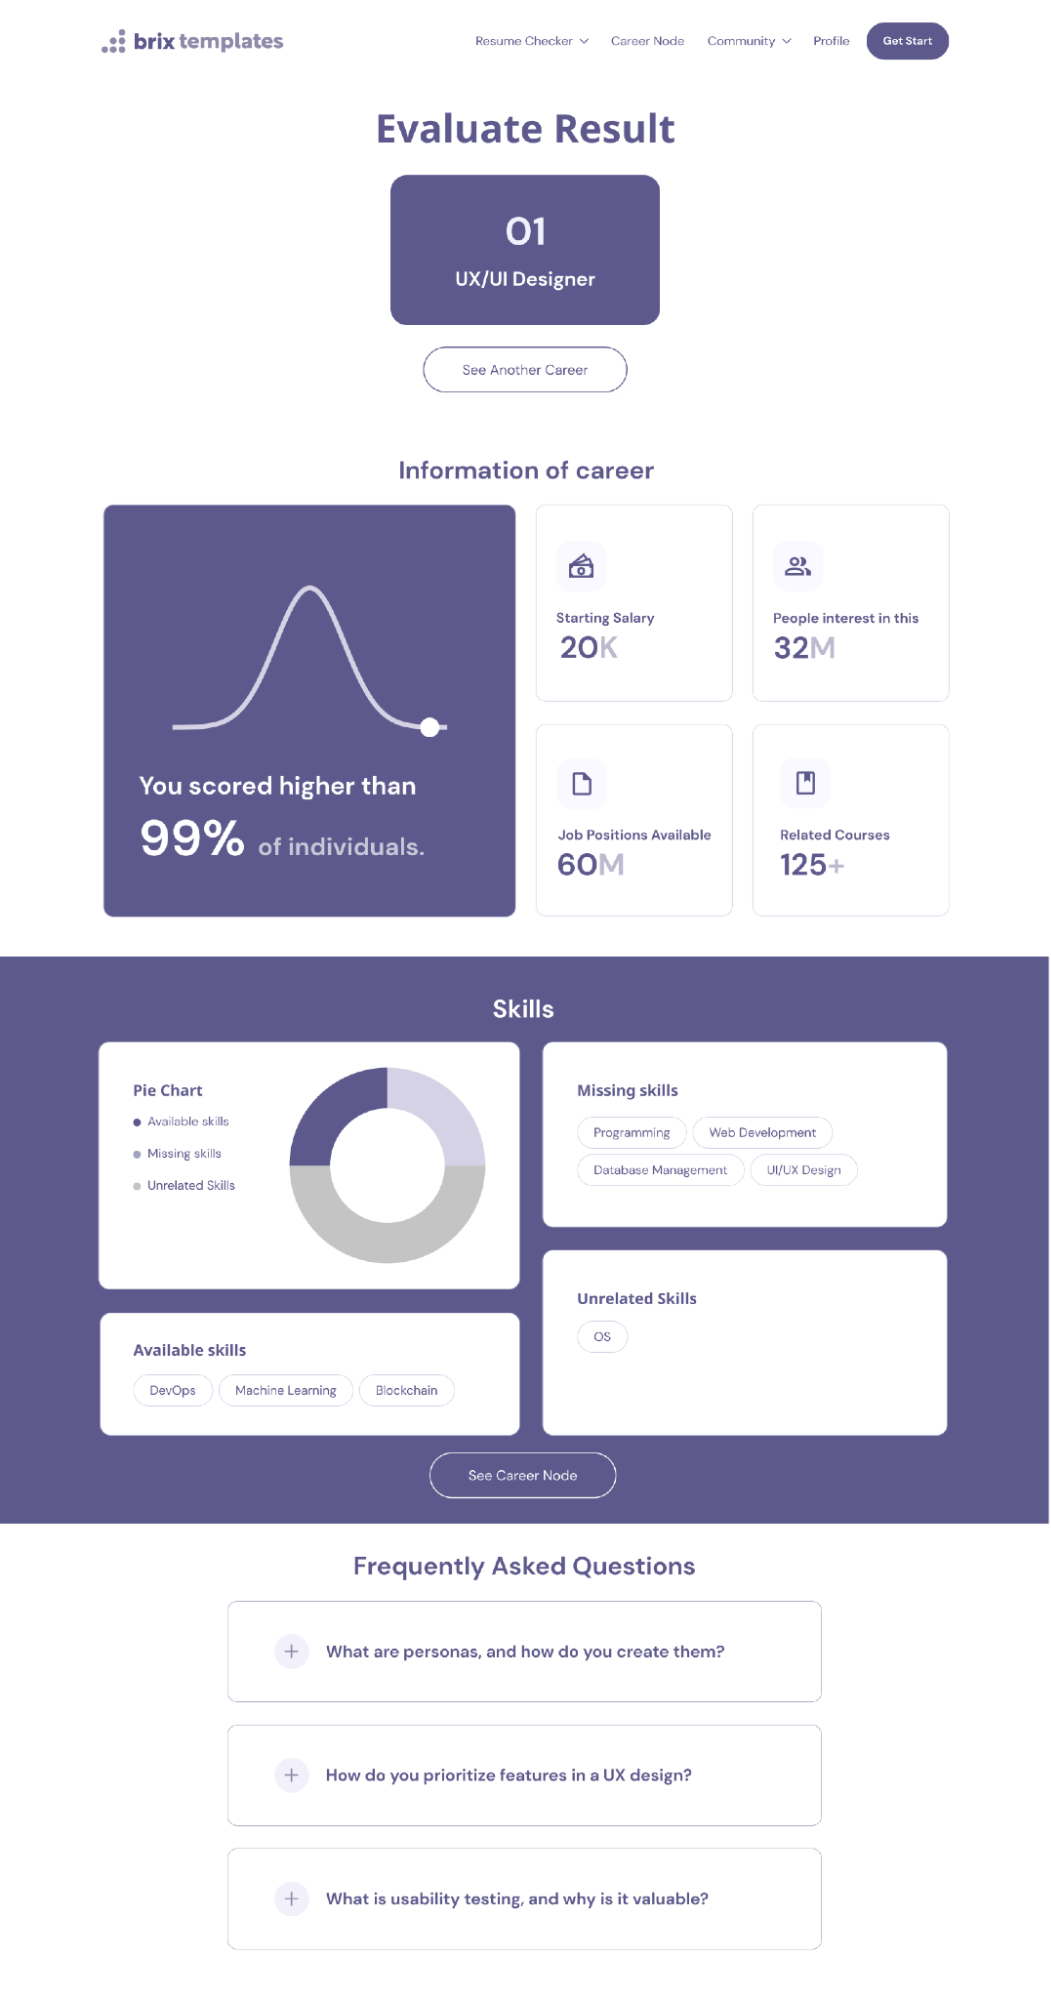
\includegraphics[width=8cm]{./figure/figure_wireframe_table3_mainpage1.png}}
              \caption{\centering หน้าแสดงข้อมูลเชิงลึกของอาชีพ}\label{fig:wireframe3_1}
          \end{figure}
\end{itemize}

\subsection {Career Node}
Career Node เป็นฟีเจอร์ที่ช่วยให้ผู้ใช้ได้เห็นภาพชัดเจนมากขึ้นเกี่ยวกับทักษะที่ต้องใช้ในอาชีพต่าง ๆ โดยจะนำเสนอข้อมูลนี้ในรูปแบบของโหนดหรือโครงสร้างเครือข่ายซึ่งช่วยให้ข้อมูลสามารถสืบค้นและเข้าใจได้ง่ายและรวดเร็ว\begin{itemize}
    \item หน้าหลัก
          \begin{figure}[H]\centering
              \setlength{\fboxrule}{0.2mm} % can define this in the preamble
              \setlength{\fboxsep}{0.5cm}
              \fbox{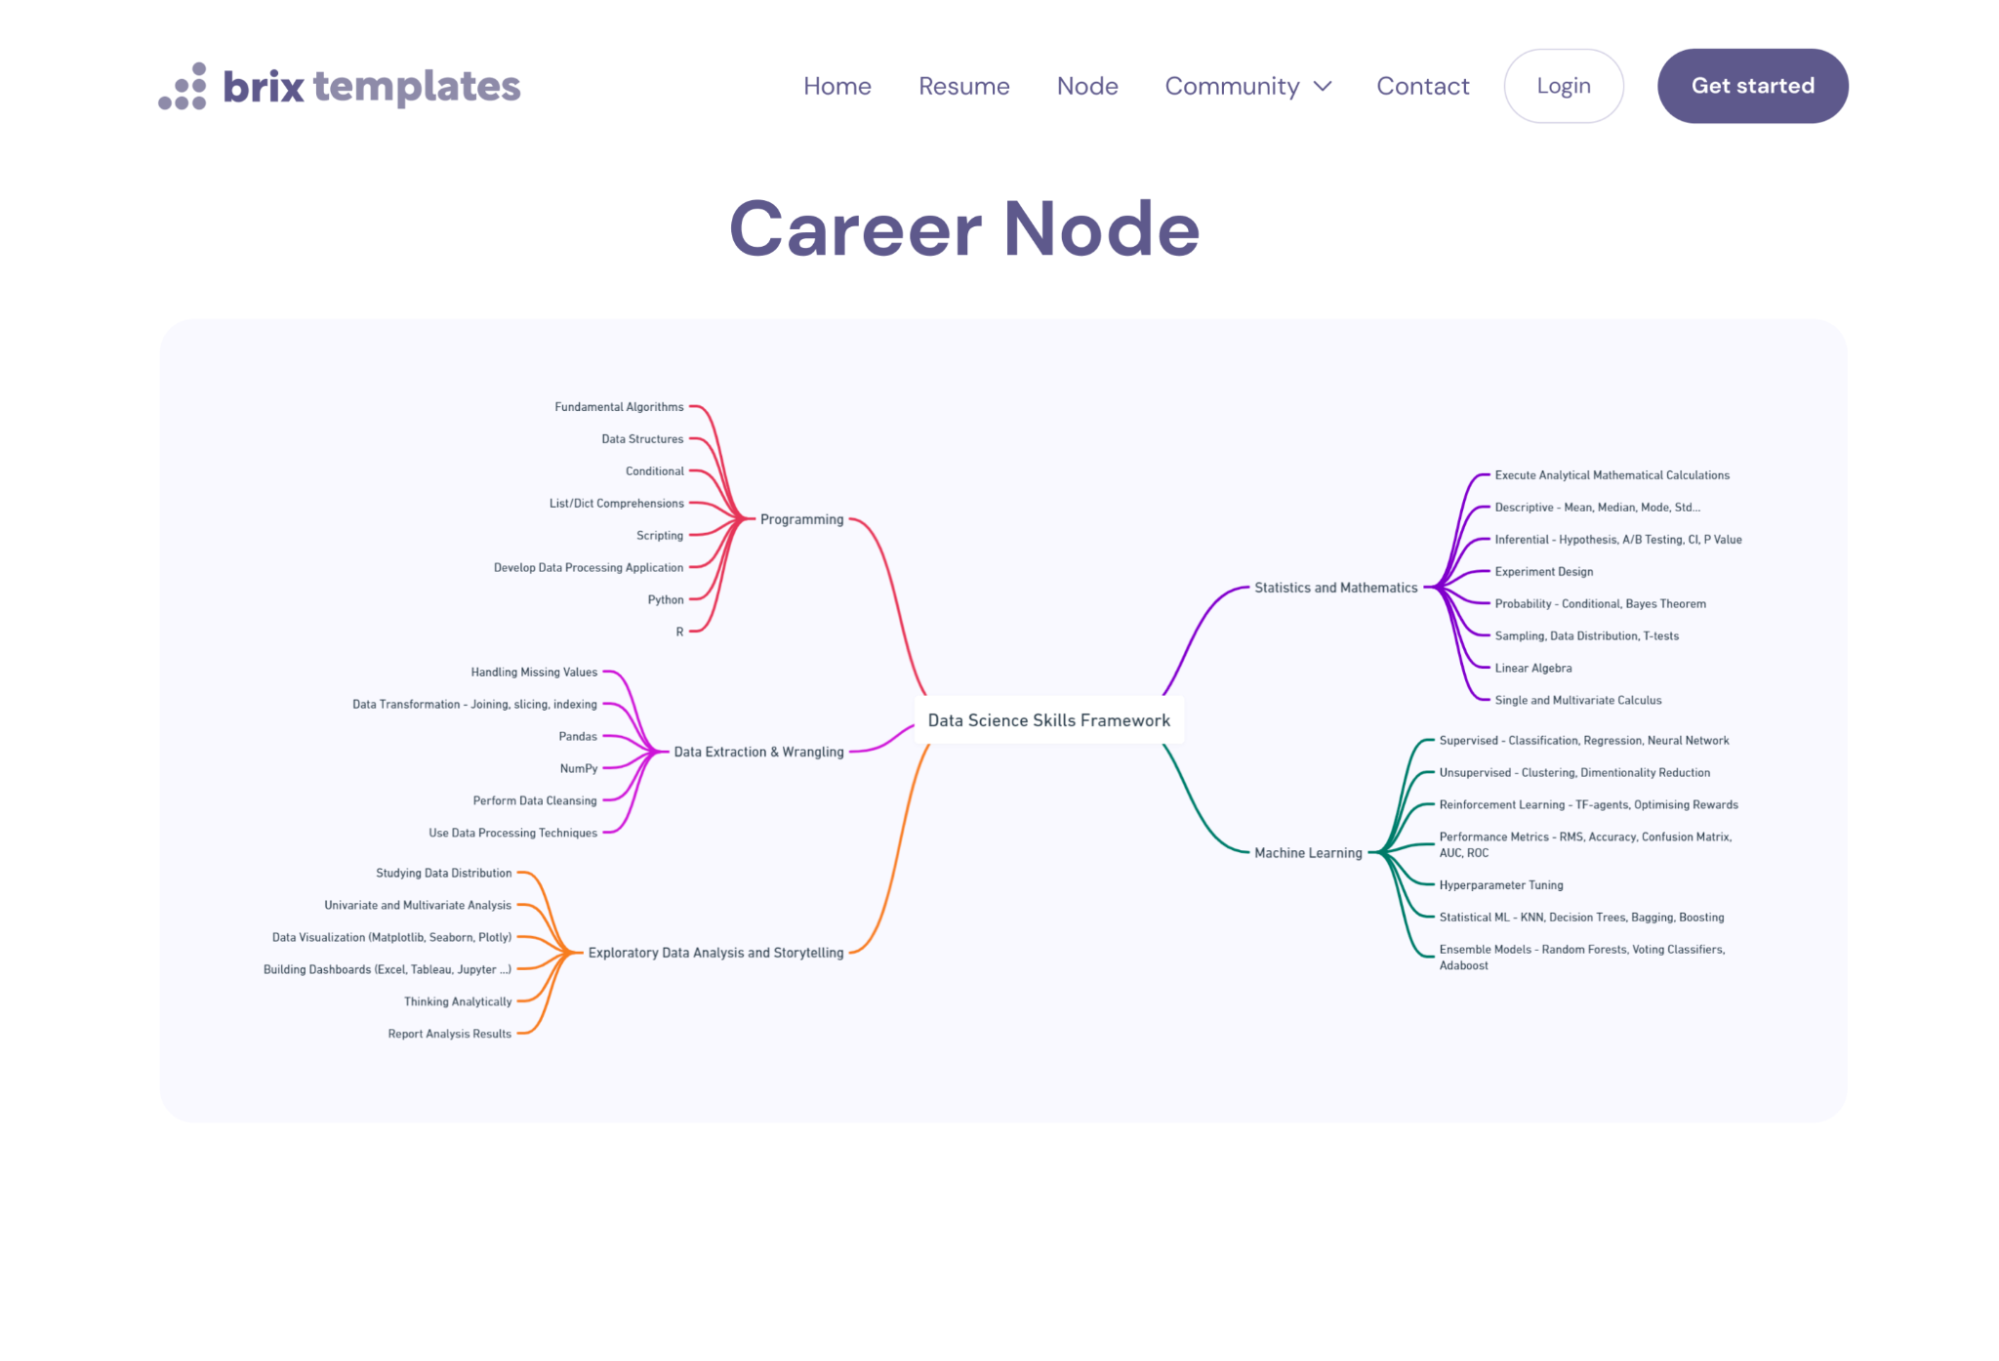
\includegraphics[width=10cm]{./figure/figure_wireframe_table4_mainpage1.png}}
              \caption{\centering หน้าแสดงทักษะที่ใช้ในสายอาชีพ}\label{fig:wireframe4_1}
          \end{figure}
\end{itemize}

\subsection {Community}
Community เป็นฟีเจอร์ที่เสริมสร้างพื้นที่สำหรับการแลกเปลี่ยนข้อมูลและความคิดเห็นระหว่างสมาชิกในระบบ โดยผู้ใช้สามารถเข้ามาสร้างและตั้งกระทู้เพื่อนำเสนอความรู้, ประสบการณ์, หรือสนทนาเกี่ยวกับหัวข้อที่น่าสนใจ\begin{itemize}
    \item หน้าหลัก
          \begin{figure}[H]\centering
              \setlength{\fboxrule}{0.2mm} % can define this in the preamble
              \setlength{\fboxsep}{0.5cm}
              \fbox{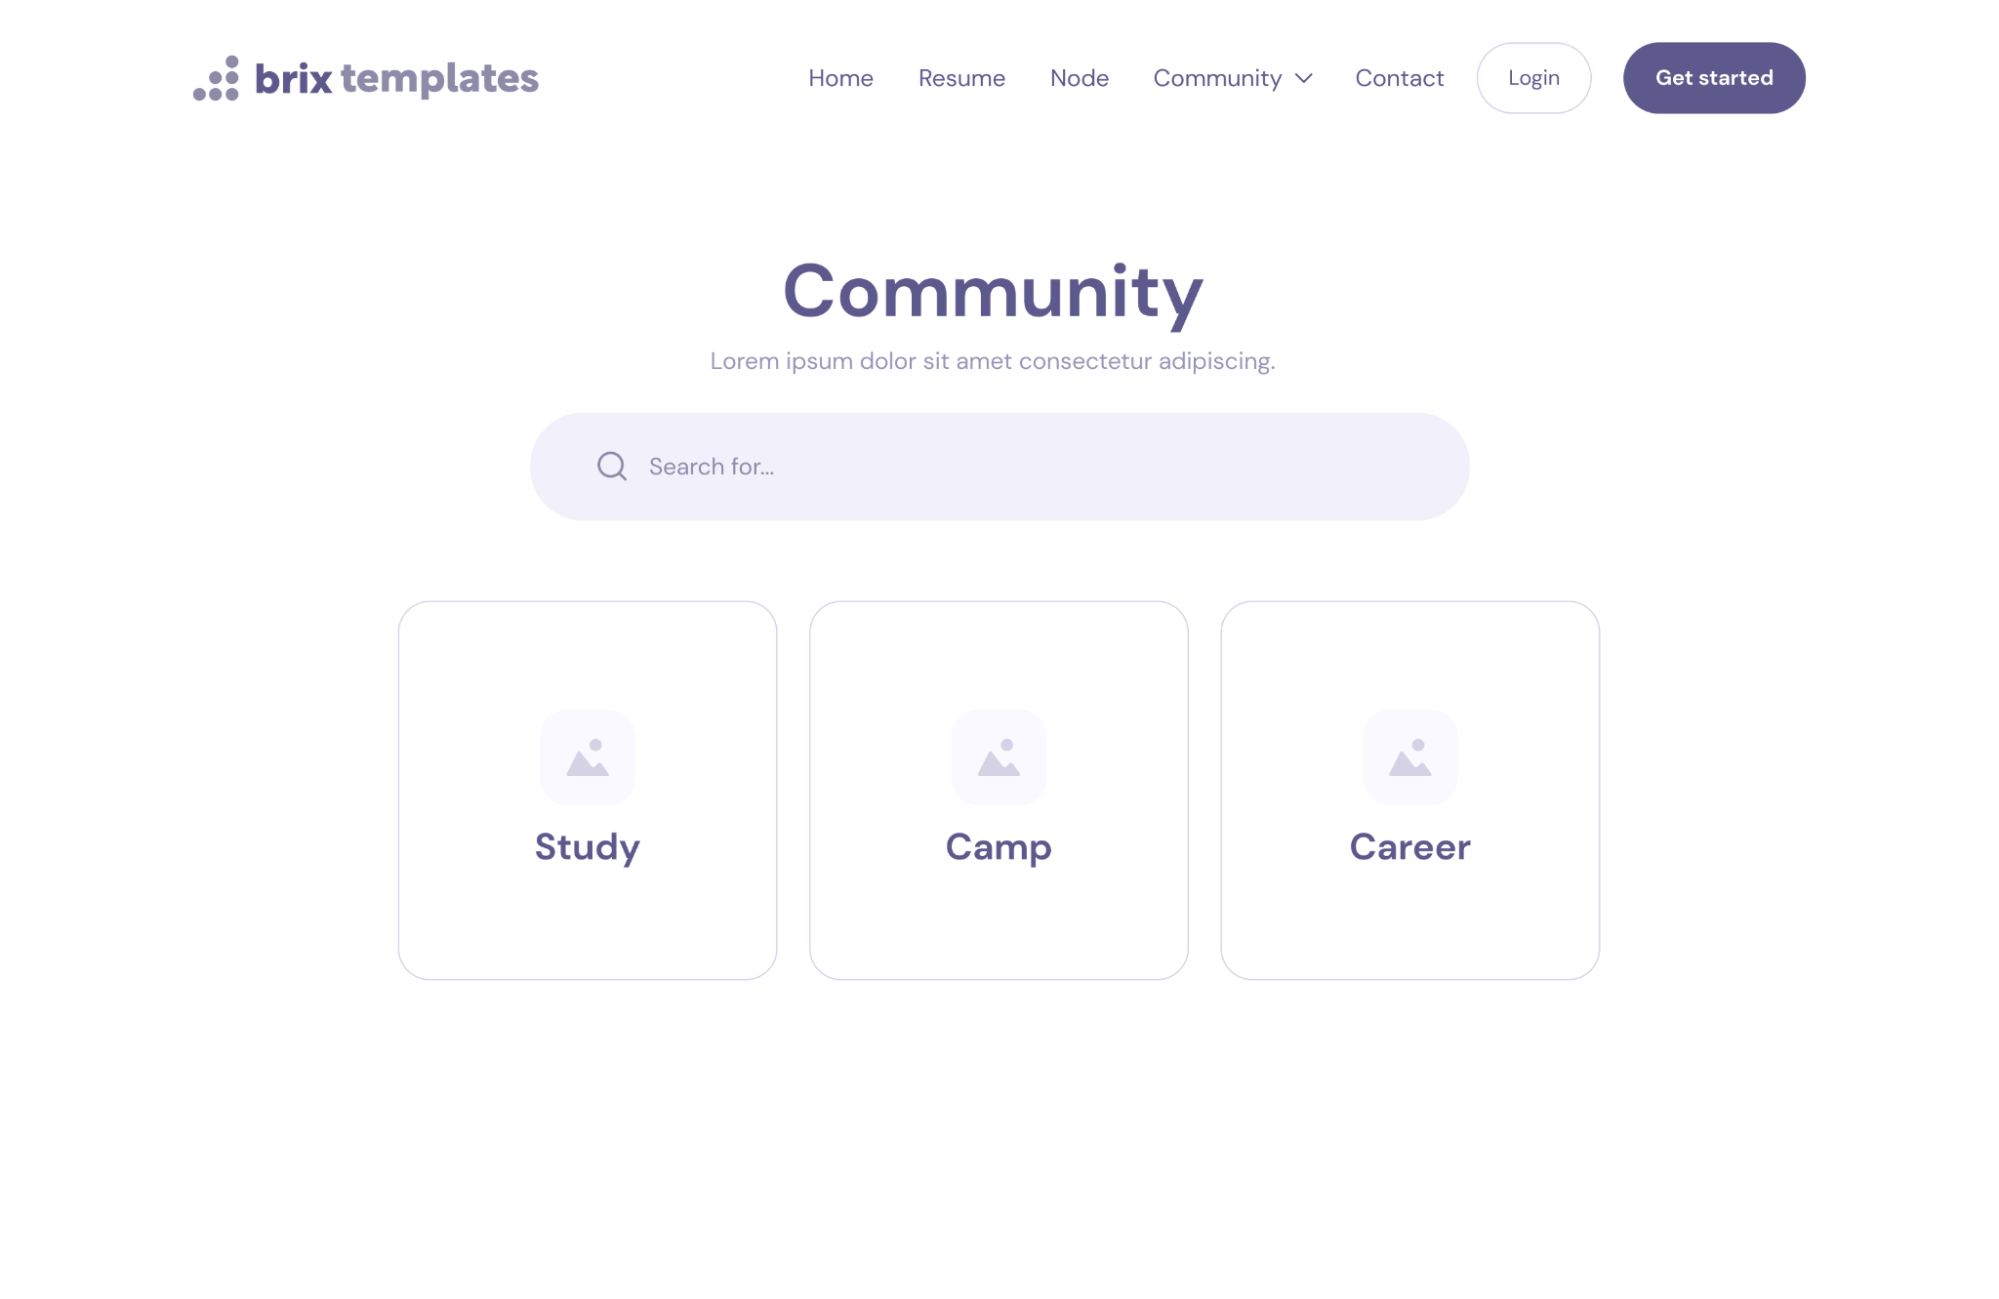
\includegraphics[width=10cm]{./figure/figure_wireframe_table5_mainpage1.png}}
              \caption{\centering หน้าเลือกหมวดหมู่กของกระทู้}\label{fig:wireframe5_1}
          \end{figure}
          \begin{figure}[H]\centering
              \setlength{\fboxrule}{0.2mm} % can define this in the preamble
              \setlength{\fboxsep}{0.5cm}
              \fbox{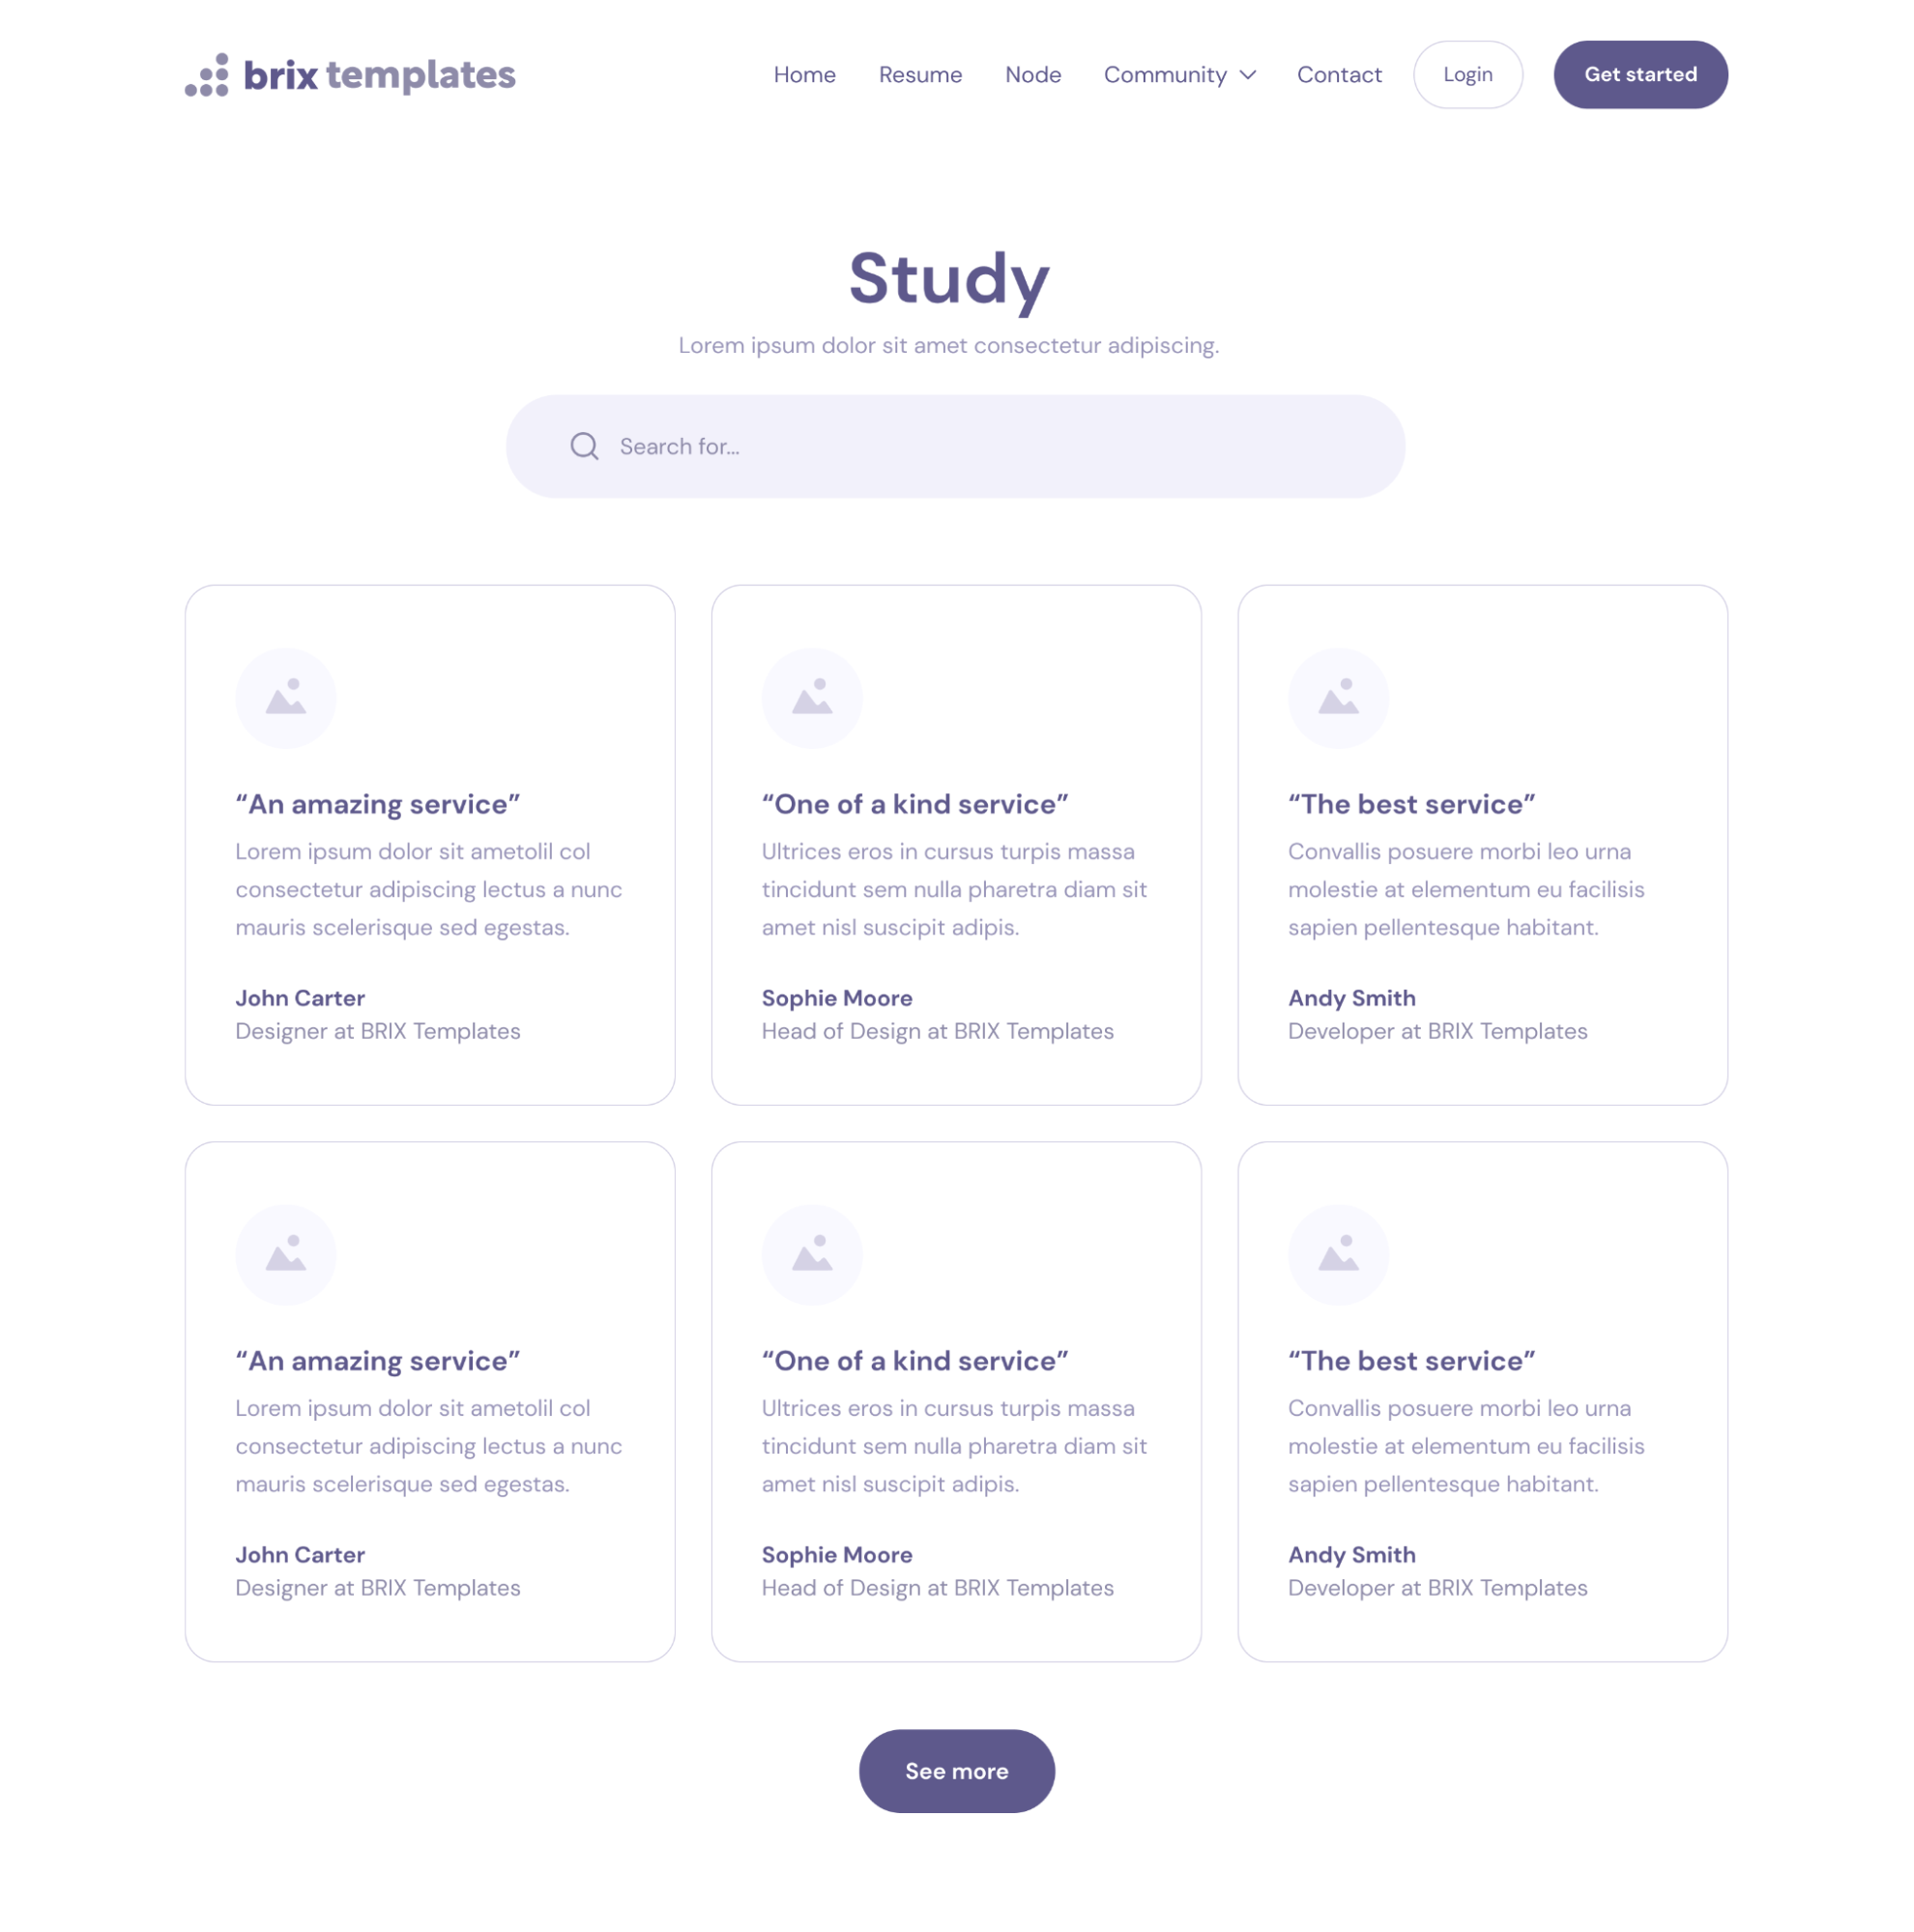
\includegraphics[width=10cm]{./figure/figure_wireframe_table5_mainpage2.png}}
              \caption{\centering หน้าแสดงรายการกระทู้}\label{fig:wireframe5_2}
          \end{figure}

          \begin{figure}[H]\centering
              \setlength{\fboxrule}{0.2mm} % can define this in the preamble
              \setlength{\fboxsep}{0.5cm}
              \fbox{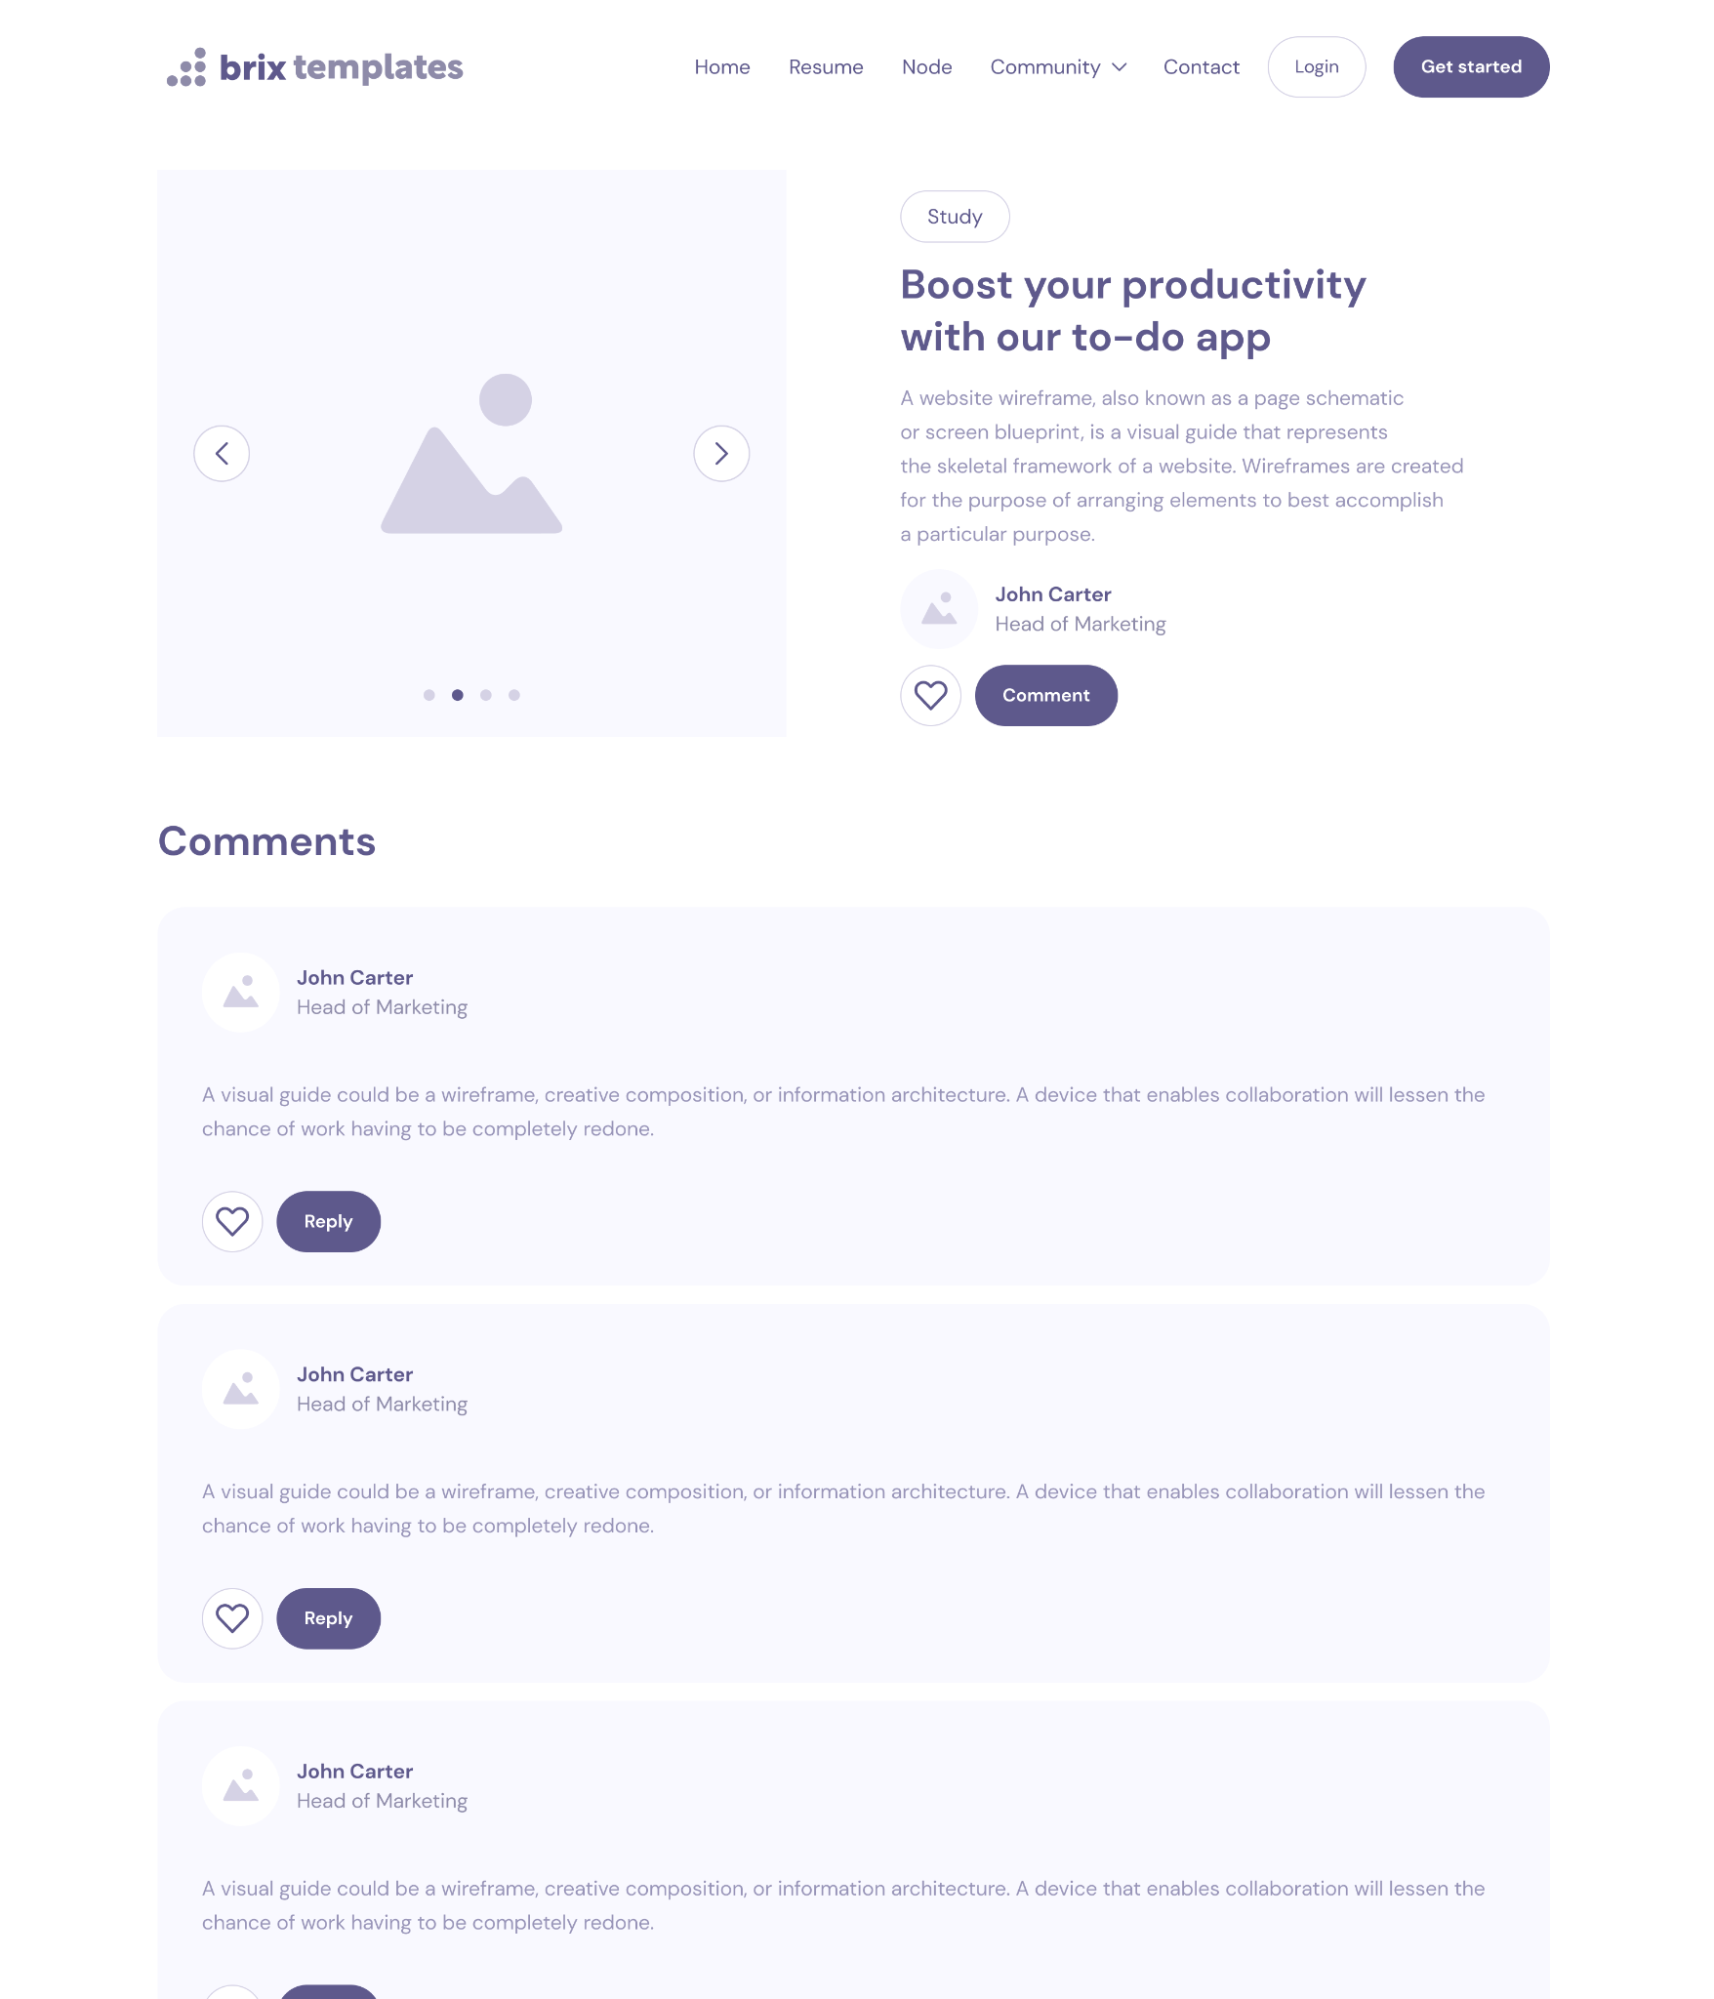
\includegraphics[width=10cm]{./figure/figure_wireframe_table5_mainpage3.png}}
              \caption{\centering หน้าแสดงรายละเอียดของกระทู้}\label{fig:wireframe5_3}
          \end{figure}
\end{itemize}
